\documentclass[11pt,a4paper]{article}

\usepackage{Act}
\usepackage{listings}

\begin{document}
\input{\detokenize{/home/fenarius/Travail/Cours/fabricenativel.github.io/latex/Macros.tex}}

\pythonmode

\PNSI{Programmation en Python}{\Pre}\vspace{0.2cm}

\Sauvegarde{DS2}

\Exo{Des carrés !}{} \\
On considère le programme Python ci-dessous :
\begin{lstlisting}
import turtle

papier = turtle.Screen()
crayon = turtle.Turtle()
crayon.pensize(3)
    
def carre_rempli(cote,couleur):
    crayon.fillcolor(couleur)
    crayon.begin_fill()
    crayon.forward(cote)
    crayon.left(90)
    crayon.forward(cote)
    crayon.left(90)
    crayon.forward(cote)
    crayon.left(90)
    crayon.forward(cote)
    crayon.left(90)
    crayon.end_fill()

# A laisser à la fin
ecran.exitonclick()
\end{lstlisting}

\QListe
\item La fonction {\tt carre\_rempli} permet de tracer un carré dont on donne le côté et la couleur de remplissage. Le carré est tracé à partir de son coin inférieur gauche.
    \SQListe
        \item En utilisant cette fonction, écrire un programme permettant de tracer les carrés suivants (les couleurs respectives sont \textit{"white"} et \textit{"gray"}) : 
        \begin{center}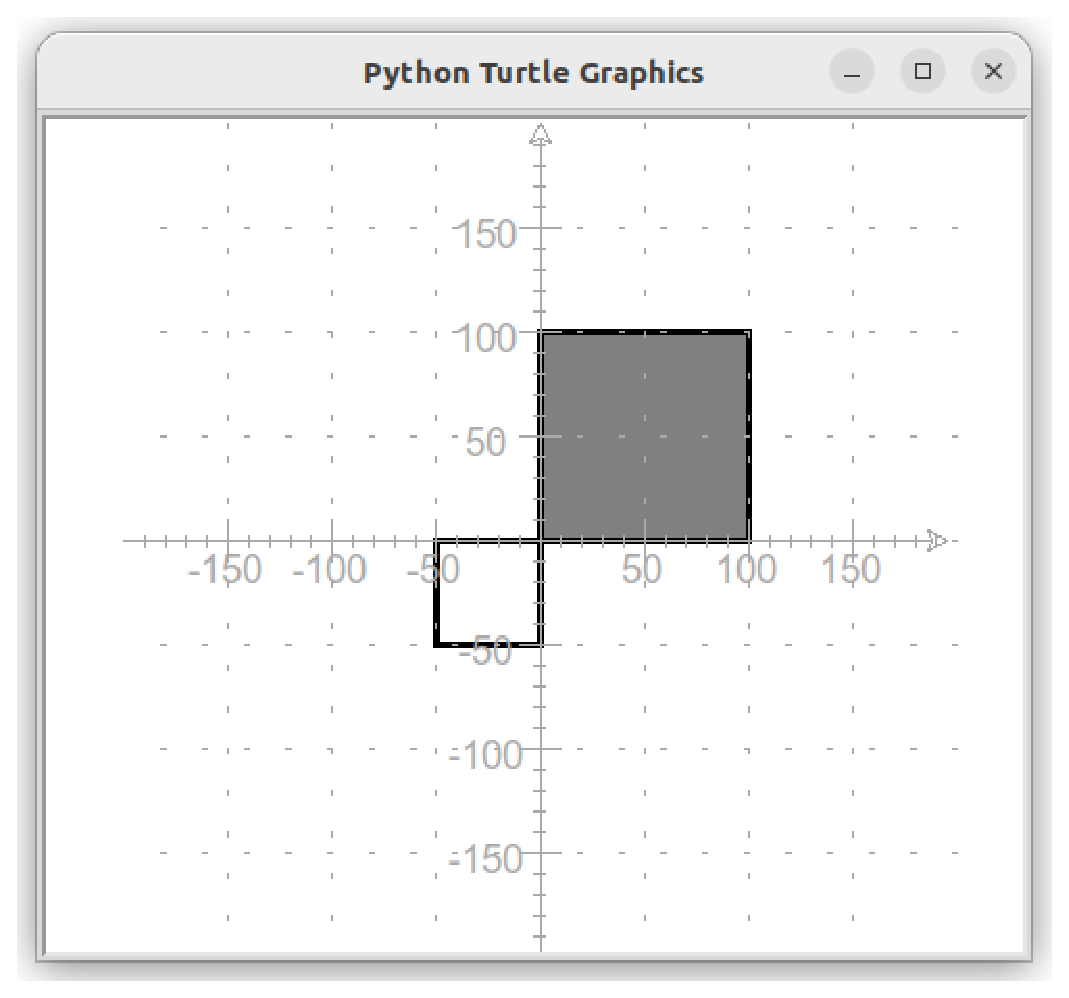
\includegraphics[width=180px]{ipt1-1.eps}\end{center}
        \item Le code de cette fonction contient des instructions qui se répètent, le réécrire en utilisant une boucle {\tt for}. 
    \FinListe
\item Ligne de carrés
    \SQListe
        \item Ecrire une fonction {\tt ligne\_carres} qui prend en argument un entier {\tt n}, une longueur {\tt cote} et une couleur de remplissage {\tt couleur} et qui trace une ligne de {\tt n} carrés de côtés {\tt cote} rempli avec la couleur {\tt couleur}. Par exemple voici le résultat de l'appel {\tt ligne\_carres(8,25,"lightgray")} lorsque la tortue se trouvait en {\tt (0,0)} :
        \begin{center}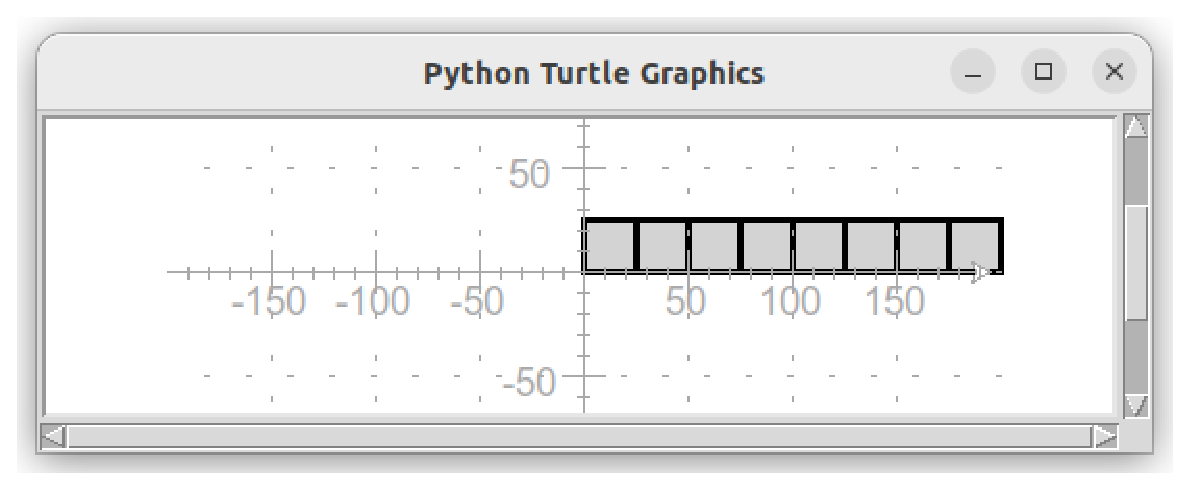
\includegraphics[width=180px]{ipt1-2.eps}\end{center}
        \item Modifier le code de la fonction {\tt ligne\_carres}, cette fonction prend un paramètre supplémentaire {\tt m} et le m-ième carré de la ligne est rempli avec la couleur \textit{white}. Par exemple voici le résultat de l'appel {\tt ligne\_carres(8,25,"lightgray",3)} (le paramètre supplémentaire {\tt m} a la valeur 3 donc le 3ème carré est rempli en blanc.)
        \begin{center}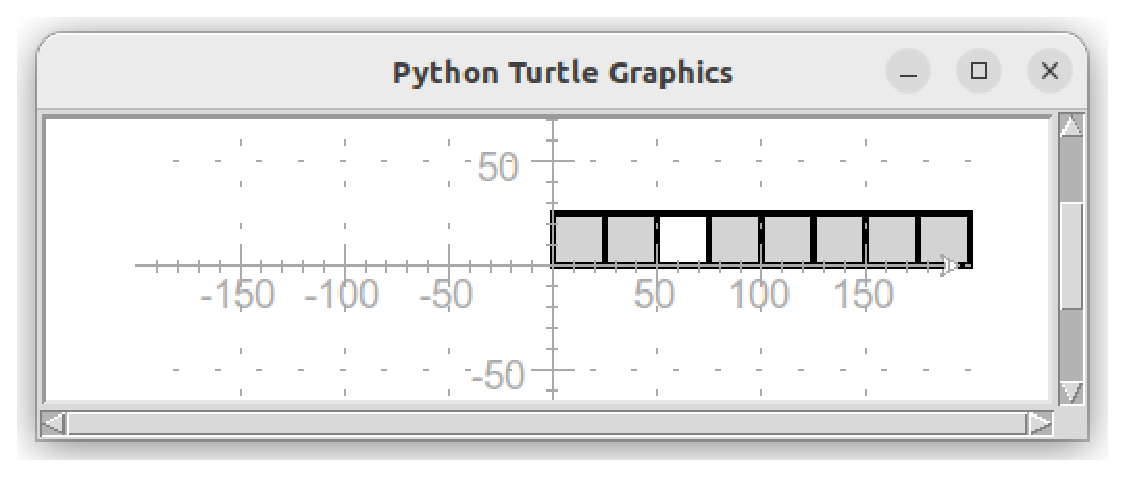
\includegraphics[width=180px]{ipt1-3.eps}\end{center}
        \item En utilisant cette fonction écrire un programme permettant de tracer la figure suivante :
        \begin{center}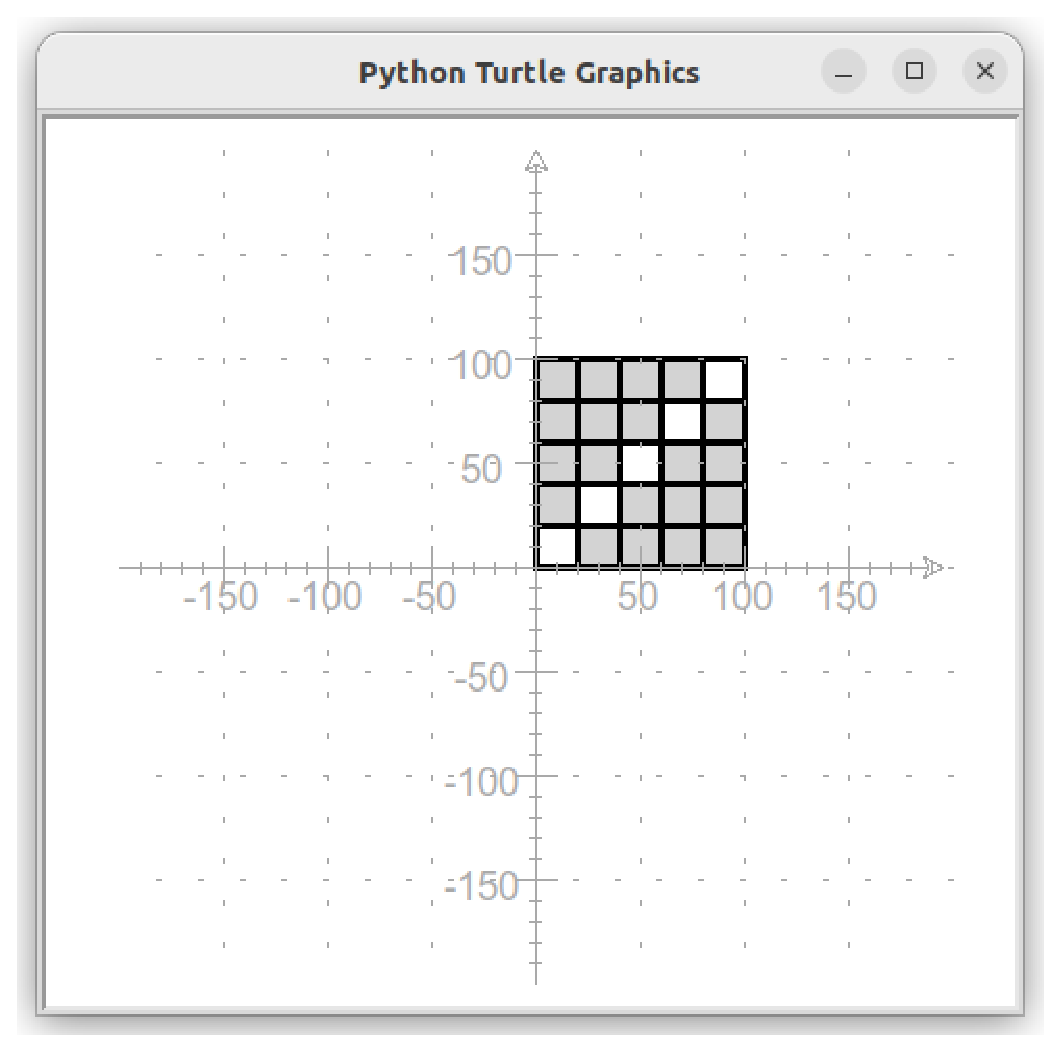
\includegraphics[width=180px]{ipt1-4.eps}\end{center}
    \FinListe
\FinListe

\vspace{0.2cm}

\Exo{Un arbre}{} \\
Pour simplifier le dessin d'un arbre, on dessine un rectangle pour le tronc et un disque pour le feuillage.
Ecrire une fonction {\tt dessine\_arbre} qui prend en les dimensions du rectangle formant le tronc et le rayon du cercle formant le feuillage ainsi que leurs couleurs de remplissage et trace l'arbre correspondant.\\
Par exemple {\tt dessine\_arbre(20,100,40,"brown","green")} dessine l'arbre ayant un tronc de 20 sur 100 en marron et un feuillage de rayon 40 en vert.
A titre d'exemple, on montre ci-dessous le résultats de trois appels à {\tt dessine\_arbre} (la tortue a été correctement positionnée avant chaque appel).
\begin{center}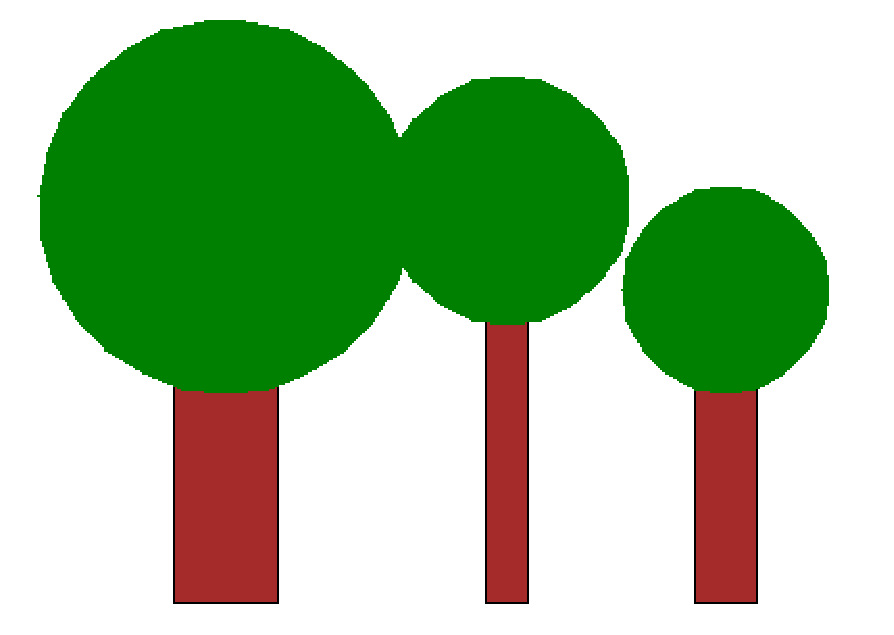
\includegraphics[width=180px]{ipt1-5.eps}\end{center}
\aide \; Pour placer le centre du cercle formant le feuillage, on a choisi de se placer ici à une hauteur des deux tiers du tronc et au milieu de celui ci.

\end{document}

